\documentclass[11pt]{scrartcl}
\newcommand{\crucial}[1]{\textbf{\sffamily\large\color{red} #1}}

\providecommand{\CC}{\mathbb C}
\providecommand{\RR}{\mathbb R}
\providecommand{\dang}{\measuredangle} %% Directed angle
\providecommand{\dg}{^\circ}
\providecommand{\half}{\frac{1}{2}}
\providecommand{\inv}{^{-1}}
\providecommand{\ol}{\overline}
%%% Load packages
\usepackage{amsmath,amssymb}
\usepackage{graphicx}
\usepackage[usenames,dvipsnames,svgnames]{xcolor}
\usepackage{hyperref}
\usepackage[obeyFinal,textsize=scriptsize,shadow]{todonotes}
\usepackage{mathtools}
\usepackage{microtype}

\usepackage{fontspec}
% https://tex.stackexchange.com/a/572220/76888
\directlua{luaotfload.add_fallback
  ("evans_fallbacks",
    {
      "Noto Serif CJK SC:style=Regular;",
    }
  )}
\setmainfont{lmroman10-regular}[
  BoldFont=lmroman10-bold,
  ItalicFont=lmroman10-italic,
  BoldItalicFont=lmroman10-bolditalic,
  SlantedFont=lmromanslant10-regular,
  BoldSlantedFont=lmromanslant10-bold,
  SmallCapsFont=lmromancaps10-regular,
  RawFeature={fallback=evans_fallbacks}
]
\setsansfont{lmsans10-regular}[
  BoldFont=lmsans10-bold,
  ItalicFont=lmsans10-oblique,
  BoldItalicFont=lmsans10-boldoblique,
  RawFeature={fallback=evans_fallbacks}
]

%%% Colored sections
\renewcommand*{\sectionformat}%
  {\color{purple}\S\thesection\enskip}
  \renewcommand*{\subsectionformat}%
  {\color{purple}\S\thesubsection\enskip}
  \renewcommand*{\subsubsectionformat}%
  {\color{purple}\S\thesubsubsection\enskip}
  \KOMAoptions{numbers=noenddot}

%%% Title
\addtokomafont{subtitle}{\Large}
\setkomafont{author}{\Large\scshape}
\setkomafont{date}{\Large\normalsize}

%%% Page setup
\usepackage[headsepline]{scrlayer-scrpage}
\renewcommand{\headfont}{}
\addtolength{\textheight}{3.14cm}
\setlength{\footskip}{0.5in}
\setlength{\headsep}{10pt}
\ihead{\footnotesize\textbf{Evan Chen《陳誼廷》} (\today)}
\automark{section}
\chead{}
\ohead{\footnotesize\textbf{Errata for E.G.M.O.}}
\cfoot{\pagemark}


\begin{document}
\title{Errata for E.G.M.O.}
\subtitle{\url{https://web.evanchen.cc/geombook.html}}
\author{Evan Chen《陳誼廷》}
\date{Last updated \today}
\maketitle

This document contains an exhaustive list of all mistakes
that I am aware of in my textbook \emph{Euclidean Geometry in Mathematical Olympiads}.
Most are annoying but benign, but a few are substantial --- these are
\crucial{emphasized in bold sans-serif red, in a slightly larger font}.
You can send any more mistakes you find to the author at
the email on \url{evanchen.cc}.

I currently do not have any plans to create a second edition.

\begin{description}

\item[p.\  xi] append a comma after ``lectures at MOP''.
\item[p.\  xiii] change ``explain how it comes from'' to ``explain where it comes from''.
\item[p.\  xiv] second bullet, the phrase ``intersection the medians'' is missing ``of''.
\item[p.\   4] \crucial{the proof of Theorem 1.3 assumes $O$ is inside $\triangle ABC$.}
  One should do (annoyingly) the other cases by a similar argument as well.
\item[p.\   7] beneath Figure 1.3A, change ``orthocenter of $H$'' to ``orthocenter of $ABC$''.
\item[p.\   9] in Problem 1.16, change $\triangle BFD$ and $\triangle CDE$
  to $\triangle DBF$ and $\triangle DEC$.
\item[p.\  10] change $(LBC)$ to $(IBC)$ in the paragraph starting ``Because $LB=LI=LC$''.
\item[p.\  12] \crucial{Theorem 1.22, the four points could also be collinear.}
\item[p.\  12] Proposition 1.24, the isosceles triangle condition holds
  only when $A$, $B$, $C$ are not collinear.
\item[p.\  16] in problem 1.33, change ``$\angle KC=90^{\circ}$'' to ``$\angle KCB=90^{\circ}$''.
\item[p.\  17] last paragraph, change ``inscribed arcs'' to ``inscribed angles''.
\item[p.\  18] in problem 1.37, delete the word ``again'' in the definition of $Q$.
\item[p.\  18] in problem 1.37, delete the word ``again'' in the definition of $Q$.
\item[p.\  18] in problem 1.38, it would be better to say
  ``prove $I_1 I_2 C B$ is cyclic'' for clarity
  since this is the order in which the vertices actually appear.
  Also, quadrilateral $ABCD$ should be required to be convex.
\item[p.\  18] in problem 1.39, $I$ is the incenter of $\triangle ABC$.
\item[p.\  19] in problem 1.45, change ``ray $BI$'' to ``the $\angle B$-bisector''.
\item[p.\  20] in problem 1.47, change ``Let $ABC$ be triangle'' to ``Let $ABC$ be a triangle''.
\item[p.\  20] in lemma 1.48, the converse should be proven to since it is quoted on page 59.
\item[p.\  24] in problem 2.2, change $\dang BCA = \dang YZX$
  to $\dang ABC = \dang XYZ$.
\item[p.\  28] change ``immediately corollary'' to ``immediate corollary''.
\item[p.\  29] in Theorem 2.9, excise ``of Intersecting Circles'' from the theorem name.
\item[p.\  29] in proof of Theorem 2.9, change both $>0$'s to $<0$'s.
\item[p.\  30] bottom of page, ``coaxal'' should be ``coaxial''.
\item[p.\  31] in Lemma 2.13, the circles can also be tangent
  to one another at $X$ (i.e.\ the intersection is counted with multiplicity).
\item[p.\  32] near start of S2.6, ``alluded the excenter'' is missing ``to''.
\item[p.\  33] in Lemma 2.20, swap the definitions of $X$ and $D$.
  (The problem is technically correct as stated,
  but it should be consistent with Figure 2.6A.)
\item[p.\  34] in the discussion for Example 2.21,
  the definition of $O_1$ and $O_2$ is accidentally omitted (but is obvious from the figure).
\item[p.\  34] in discussion to Example 2.21, in
  ``we already know that that lines $PQ$, $RS$, and $XY$ concur at a point $X$'',
  the extraneous ``that'' and ``$X$'' should both be deleted.
\item[p.\  34] end of third paragraph in discussion to Example 2.21,
  change ``$\omega_1$ an $\omega_3$'' to ``$\omega_1$ and $\omega_3$''
  and change $O_1O_3$ to $\ol{O_2O_3}$.
\item[p.\  35] in the second set of aligned equations,
  change $O_2X^2$ to $OO_2^2$.
\item[p.\  35] very bottom of page, change ``circmuradii'' to ``radii''.
\item[p.\  37] Example 2.23, the source is Russia 2011, not 2010.
\item[p.\  39] Example 2.24, $I$ is the incenter.
\item[p.\  40] Problem 2.29, change ``six points'' to ``the six points''.
\item[p.\  40] Problem 2.30, the lines may also be pairwise parallel.
\item[p.\  46] change $\frac 11 \frac 11 \frac 11 = 1$ to $1 \cdot 1 \cdot 1 = 1$.
  (not technically wrong but quite misleading as written.)
\item[p.\  47] before figure 3.3B, change $AA_1=p$ to $AA_1=|p|$; ditto for $B_1$ and $C_1$.
\item[p.\  48] Theorem 3.8, the lines may also be pairwise parallel.
\item[p.\  49] when defining homothety, $h(P)$ must also lie on line $PO$.
\item[p.\  49] third to last line, lengths are multiplied by $|k|$.
\item[p.\  51] before Lemma, in ``this circles is called the nine-point circle'',
  change ``circles'' to ``circle''.
\item[p.\  54] third paragraph, change ``pick let'' to ``let''.
\item[p.\  55] immediately after display, $\dang BH_AO$ should be $\dang OH_AB$.
\item[p.\  56] in the Ceva application, change $\frac{BF}{FA}$ to $\frac{AF}{FB}$.
\item[p.\  57] in Problem 3.25 require $ABCD$ to be convex.
\item[p.\  59] after Problem 4.2, change $AHPK'$ to $AHK'P$.
\item[p.\  61] before Problem 4.8, the definition of $D$ is omitted (but obvious from Figure 4.2B).
\item[p.\  65] Problem 4.25, change $\frac{BM}{MC}$ to $\frac{CM}{MB}$.
\item[p.\  67] in Lemma 4.33, change the second $\omega$ to $\Omega$.
\item[p.\  68] just before Problem 4.38, change ``show'' to ``shown''.
\item[p.\  71] Problem 4.53 is missing a trailing period.
\item[p.\  76] \crucial{Theorem 5.1 is missing a factor of $\frac12$.}
\item[p.\  76] The shoelace formula is \textbf{antisymmetric}, not symmetric.
\item[p.\  89] at the start of the final paragraph in solution to Example 5.14
  change ``if and only $\theta$'' to ``if and only if $\theta$''.
\item[p.\  89] to finish example 5.14, one should also verify that $\angle A = 60\dg$
  and $\angle A = 90\dg$ actually work.
  As written, this is a proof that only $60\dg$ and $90\dg$ \emph{could} work,
  and does not mention the converse direction.
\item[p.\  92] \crucial{In Problem 5.23, when defining point $G$,
  line $HE$ should intersect $\Gamma_1$, not $\Gamma_2$.}
  Also, ``interest'' should be ``intersect'' in the first line.
\item[p.\  97] Figure 6.2A, should be $iz = -4+3i$.
\item[p.\  98] after the display, $is$ should not be in math mode.
\item[p.\  100] in the first sentence of the paragraph before Theorem 6.7,
  delete the extra repeated ``that''.
\item[p.\  101] in the proof of Example 6.10, Lemma 6.3 should be Lemma 6.5.
\item[p.\  101] in the proof of Lemma 6.12, every logical $\implies$ should
  really be a bidirectional $\iff$ for the proof to be executed correctly.
\item[p.\  103] second to last paragraph, replace ``indeed cyclic'' with ``indeed concyclic''.
  Also, $\frac{xa}{bc}$ should be $\frac{bc}{xa}$ (two changes).
\item[p.\  104] in the proof of 6.16, replace ``similar'' with ``directly similar''.
\item[p.\  105] in Problem 6.20 change ``Theorem 6.16'' to ``Theorem 6.15''.
\item[p.\  107] \crucial{The proof of the theorem
  has several issues, and is probably best to just ignore.}
  The figure 6.6B is similarly broken.
  (The result is still true.)
\item[p.\  109] Third paragraph, $A=x^2$, $B=y^2$, $C=z^2$
  should just be $a=x^2$, $b=y^2$, $c=z^2$ though this doesn't really matter.
\item[p.\  111] the last expression should actually be negated.
\item[p.\  112] in the second displayed line, change $y^2+x^2z/y$ to $-y^2+x^2z/y$.
  In the fourth, change the second $y^2/z^2$ to $z^2/y^2$.
  In the ninth, change the second $y^2/z^2$ to $z^2/y^2$.
  In the penultimate display (starting from $b_1$), change the period to a comma.
\item[p.\  113] in the definition of $M_2$, change $DH_A$ to $AH_A$.
\item[p.\  114] Solution to Example 6.27, the $a$ in the numerator of $a'$ should be $\bar a$.
  Follow through with the rest of the solution.
\item[p.\  114] Solution to Example 6.27, near the end, negate all terms of
  $\sum (a \ol b - a \ol c + c \ol a - b \ol a)$
\item[p.\  117] in Problem 6.38 (which starts on the previous page), the similarity
  $\triangle DPO \sim \triangle PEQ$ should be a direct similarity.
\item[p.\  115] In lemma 6.30, ``chord $AB$'' should technically be ``line $AB$''.
\item[p.\  120] change $PAB$ to $PXY$.
\item[p.\  121] change ``his idea'' to ``this idea''.
\item[p.\  121] ``delimited with colons'' should be
  ``delimited with commas''.
\item[p.\  125] at the end of the proof of Theorem 7.13,
  change ``occurs only when'' to ``occurs precisely when'',
  since the statement is if-and-only-if.
\item[p.\  126] in Theorem 7.14 and proof, $|PQ|^2$ should technically be just $PQ^2$.
\item[p.\  130] in the proof of Example 7.20, change $(bs:b:2b)=(bs:b:c)$ to $(bt:b:2b)=(bt:b:c)$.
  Omit $s=t/b$ which is never used.
\item[p.\  132] in the proof of Example 7.20, change $C = (0, 0, 1)$ to $D = (0, 0, 1)$.
\item[p.\  132] in the last display change $\angle FAD$ to $\angle KAD$.
\item[p.\  133] Proposition 7.21, last display, change $S_a$ to $S_A$.
\item[p.\  134] in the display before Theorem 7.25,
  change $\overrightarrow{HO}$ to $\overrightarrow{OH}$.
\item[p.\  134] in Theorem 7.25, change
  $\overrightarrow{AO}$, $\overrightarrow{BO}$, $\overrightarrow{CO}$ to
  $\overrightarrow{OA}$, $\overrightarrow{OB}$, $\overrightarrow{OC}$.
  (Technically, the original theorem is still true,
  but this way the notation is consistent with preceding paragraph.)
\item[p.\  135] in Example 7.26, change both $\overrightarrow{PA}$'s to $\overrightarrow{AP}$'s,
  and $\overrightarrow{AO}$ to $\overrightarrow{OA}$.
\item[p.\  136] very top, $c=AE$ should be $c=AC$.
\item[p.\  137] in the definition of bolded term ``homogeneous coordinates'',
  replace $(x,y,z)$ with $(x:y:z)$ for clarity.
\item[p.\  137] in Example 7.28, change ``$\overline{BC}$'' to ``segment $BC$''.
\item[pp.\  137--138] the solution to 7.28 only addresses one direction
  though the other follows similar.
\item[p.\  138] eighth line from top, change $AD:AC$ to $AD:CD$.
\item[p.\  139] start of page, delete ``determinants and''.
\item[p.\  139] Solution 7.29, change the first display to
  $0 = c^2(t-1) + (a^2-b^2) \implies t = \frac{c^2+b^2-a^2}{c^2}$.
\item[p.\  140] in the second display, $x+y$ should be $x-y$.
\item[p.\  141] $H = (S_{BC},S_{CA},S_{AB})$ should have
  colons and not commas.
\item[p.\  141] change ``$P = \left(x' : y' : z'\right) = \left(x' : y' : -S_{AB}\right)$''
  to ``$P = \left(x : y : z\right) = \left(x' : y' : -S_{AB}\right)$'',
  ``$0 = x' - y' + \left( \frac{S_{AC}-S_{BC}}{S_{AB}} \right) z'$''
  to ``$0 = x - y + \left( \frac{S_{AC}-S_{BC}}{S_{AB}} \right) z$'',
  ``$a^2 y'z' + b^2 z'x' + c^2 x'y' = 0$''
  to ``$a^2 yz + b^2 zx + c^2 xy = 0$''.
\item[p.\  142] very top, in $a^2=S_{AB}+S_{AC}$, change LHS to $a^2S_A$.
  Also, the rest of the solution is wrong, since a factor of two is dropped in the first display.
\item[p.\  145] in Problem 7.44, $C_1$ should be different from $A$ or $B$.
\item[p.\  145] Problem 7.50 should clarify that $E \neq B$ and $F \neq C$.
\item[p.\  146] \crucial{Problem 7.52, change $\angle PCB$ to $\angle PBC$.}
\item[p.\  144] second line of 7.42, change ``tangency points'' to ``tangency point''.
\item[p.\  149] second paragraph of 8.1, change ``three ordinary points''
  to ``three noncollinear ordinary points''.
\item[p.\  149] third paragraph of 8.1, change $R$ to $r$.
\item[p.\  150] in Lemma 8.1, replace ``tangents from $A^\ast$'' with ``tangency points from $A^\ast$''.
\item[p.\  151] at start of 8.2, in ``simplest example is a just a line'', delete the extra ``a''.
\item[p.\  151] immediately before figure, add a period after 8.2A.
\item[p.\  151] the proof of Proposition 8.5 only shows that $\ell^\ast$ is a subset of the circle
  $\gamma$, and some bijection-like comment is technically needed to finish.
\item[p.\  152] right before theorem 8.7,
  change ``the following lemma'' to ``the following theorem''.
\item[p.\  153] in Theorem 8.7(c), ``another circle'' does not imply distinctness.
  (To be precise, circles invert to themselves if and only if they are orthogonal.)
\item[p.\  153] Lemma 8.11 is misnamed, and should be ``inverting the circumcircle''
  or ``inverting \emph{around} the incircle''.
\item[p.\  154] in Example 8.12 require $ABCD$ to be convex.
\item[p.\  154] in Step 6, change ``$WXYZ$ is concyclic'' to ``$W$, $X$, $Y$, $Z$ are concyclic''.
\item[p.\  155] first bullet, delete the extra comma.
\item[p.\  156] change ``they are \textbf{orthogonal}'' to ``$\omega_1$ is \textbf{orthogonal} to $\omega_2$'',
  and insert ``We therefore say that they are orthogonal if one is orthogonal to the other.'' after the last sentence of the first paragraph.
\item[p.\  158] $\Gamma_{AB}^\ast$ and $\Gamma_{AC}^\ast$ are rays, not lines (in both figure and text).
  Also, $\omega_0$ is a semicircle rather than a circle.
\item[p.\  159] second line of Example 8.15,
  change ``tangent to $\omega$ at $T$'' to ``tangent to $\Omega$ at $K$''.
  Also, in the second paragraph of the proof, change the last $\Gamma$ to $\Omega$.
\item[p.\  159] \crucial{in Lemma 8.16, change ``fixes $B$ and $C$'' to ``swaps $B$ and $C$''.}
\item[p.\  162] item 5 of list, change $G_1$ to $G_1^\ast$.
  Also $G^\ast$ in the first paragraph of the solution.
\item[p.\  162] in the first sentence of the solution,
  change ``the intersection'' to ``the second intersection''.
\item[p.\  163] switch $C^\ast$ and $D^\ast$ in the diagram 8.7D.
\item[p.\  163] step 3, change $BS^\ast$ to $BC^\ast$.
\item[p.\  164] switch $R^\ast$ and $S^\ast$ in the diagram 8.7E.
\item[p.\  164] change $BX^\ast G^\ast$ in the display to $BXG^\ast$
\item[p.\  164] switch $S^\ast$ and $R^\ast$ in the diagram.
\item[p.\  164] insert ``is'' between ``it isosceles''.
\item[p.\  166] Problem 8.26 is BAMO 2008/4, not BAMO 2080/6.
\item[p.\  167] Problem 8.34 requires $A$, $B$, $C$, $D$ to be distinct.
\item[p.\  167] Problem 8.36, ``circumcircle'' is misspelled.
\item[p.\  171] Theorem 9.2, change ``$\ol{AB}$ and $\ol{XY}$'' to ``segments $AB$ and $XY$''.
\item[p.\  171] there's some abuse of notation in that $P(A,B;X,Y)$
  was technically only defined for $ABXY$ collinear,
  but the intention is that $P(A,B;X,Y)$ refers to the cross ratio obtained
  from the four lines concurrent at $P$.
\item[p.\  171] ``if one of the angles'' would be clearer as ``if any of the
  angles'', when defining the sign of $(a,b;x,y)$.
\item[p.\  172] in the paragraph before Figure 9.2C,
  ``(and vice versa)'' is redundant, it is in the previous sentence already.
\item[p.\  173] in Problem 9.3, the points should also be collinear.
\item[p.\  173] in Problem 9.4, add $k \neq 0$.
\item[p.\  173] 7th line of Section 9.3, in ``we present four configurations'',
  change ``four'' to ``five''.
\item[p.\  174] display in proof of Lemma 9.9, change $(A,B;Q,P)$ to $(A,B;P,Q)$.
\item[pp.\  174--175] in names of Lemmas 9.11-9.12,
  change ``Induces'' to ``Induce''.
\item[p.\  175] ``directed form *of* Ceva's theorem''.
\item[p.\  176] in Problem 9.14, delete ``and Lemma 9.18'' (and ``proofs'' to ``proof'').
\item[p.\  177] in Lemma 9.18, change ``implies'' to ``imply''.
\item[p.\  178] in the proof of Theorem 9.19, change $\angle CAY = \angle YBC$ to $\angle ACY = \angle YCB$.
\item[p.\  179] top of page, first sentence, $\ell$ is allowed to pass through $O$.
\item[p.\  179] in proof of Proposition 9.24, La Hire is used implicitly at the end
  to get $Q$ lies on the polar of $P$ iff $P$ lies on the polar of $Q$.
\item[p.\  181] in Lemma 9.27, change ``pole'' to ``polar'' (two instances).
\item[p.\  184] \crucial{in Theorem 9.33,
  uniqueness is not true for (b) or (c).
  The last sentence is also wrong as written.
  The correct sentence is: if the \emph{circumcircle} of a cyclic quadrilateral is sent to a circle,
  then so is the cross ratio of the cyclic quadrilateral.}
\item[p.\  184] in Example 9.34, swap the definitions of $P$, $Q$.
\item[p.\  184] in solution to Example 9.34,
  replace the definition of $P'$ with $P' = \ol{A'B'} \cap \ol{C'D'}$.
\item[p.\  187] in solution to 9.38, $I_A$ is the $A$-excenter (of course).
\item[p.\  189] in Solution 1, $T$ should be $\ol{AA} \cap \ol{CR}$.
\item[p.\  190] immediately before problems, $P$ is the point at infinity along $\ol{AC}$ instead.
\item[p.\  191] the source ``Singapore TST'' of Problem 9.43 is a bit dubious.
  It seems to have come from \url{https://aops.com/community/p3491333},
  which suggests the year is 2008,
  but is not present in \url{https://aops.com/community/c3691_2008_singapore_team_selection_test}.
  Go figure.
\item[p.\  191] in Problem 9.47, last line of problem statement,
  change ``circumference'' to ``circumcircle''.
\item[p.\  191] in Problem 9.48, the definition of $E$ and $F$ are swapped from
  the original source, though this has no bearing on the problem.
\item[p.\  192] Problem 9.54, should be the interiors of the sides, i.e.\ $A \neq D$ and $C \neq E$.
\item[p.\  193] Problem 9.58, delete the last ``again'' in definitions of $P$, $Q$.
\item[p.\  196] right after Figure 10.1B, ``similar'' would be better as ``directly similar''.
\item[p.\  198] in proof of 10.3, change ``$BC$ to $DA$'' to ``$BC$ to $AD$''.
\item[pp.\  198--$\infty$] replace ``Gauss line'' with ``Newton-Gauss line''
  everywhere --- that's the standard term, apparently.
\item[p.\  200] in third sentence of proof, add ``of'' after ``radical center''.
\item[p.\  201] Lemma 10.9, change ``though'' to ``through''.
\item[p.\  201] The complete quadrilateral $ABCD$ is cyclic if $A$, $B$, $C$, $D$ lie on a circle.
\item[p.\  202] Proposition 10.14, delete extra ``the'' before $M$.
\item[p.\  202] part (a), the latter four circles should be
  $(PAB)$, $(PCD)$, $(QAD)$, $(QBC)$.
\item[p.\  202] part (b), change ``$AB$ to $CD$'' to ``$AB$ to $DC$''
  and change ``$BC$ to $DA$'' to ``$BC$ to $AD$''.
\item[p.\  205] solution to Example 10.16 should define $O$ as the center of $\omega$,
  once it is prove that $KL K^\ast L^\ast$ is cyclic.
\item[p.\  206] problem 10.23, change ``IMO 2005/2'' to ``IMO 2005/5'',
  and ``lie of the sides'' to ``lie on the sides''.
\item[p.\  209] problem 11.5, for clarity,
  expand ``USAMTS'' as ``USA Mathematical Talent Search'',
  and require $ABCD$ to be convex.
\item[p.\  209] problem 11.6, change ``circumcenter'' to ``circumcircle''.
\item[p.\  210] problem 11.8, assume $AB \neq AC$.
\item[p.\  210] problem 11.10, change ``$PA$, $PB$, $PC$'' to ``$AP$, $BP$, $CP$''.
  Also, require $P$ to not be the orthocenter.
\item[p.\  216] in phrase ``third column from the first column'',
  change ``first'' to ``second''.
\item[p.\  217] to be extremely pedantic, what's define is a vector in $\RR^n$.
  In abstract algebra the definition of a vector is more general
  and there is not necessarily a norm or direction.
\item[p.\  218] in definition of vector addition,
  change to $\left\langle x_1+x_2, y_1+y_2 \right\rangle$.
\item[p.\  218] the misspelled ``ofter'' should be ``often''
\item[p.\  219] replace ``two vectors $v$ and $w$'' with ``two vectors $\vec v$ and $\vec w$''.
\item[p.\  219] \crucial{the dot product is not associative};
  that property does not even make sense for this operation,
  since is an operation from $\RR^n \times \RR^n \to \RR$.
\item[p.\  221] hint 8, replace ``How you can'' with ``How can you''.
\item[p.\  221] hint 12 is wrong (see page 268 correction below).
\item[p.\  222] hint 40, ``It equivalent'' is missing ``is''.
\item[p.\  222] hint 60, the inequality should be strict.
\item[p.\  221] hint 66 is wrong (see page 268 correction below).
\item[p.\  223] hint 77, replace ``$\dang CMN = \dang BMN$''
  with ``$\dang CNM = \dang BNM$''.
\item[p.\  223] hint 83, replace ``not disjoint'' with
  ``not disjoint nor neither one is contained inside the other''.
\item[p.\  223] hint 87, the inequality should be strict.
\item[p.\  223] hint 93, replace ``at least'' with ``more than''.
\item[p.\  223] hint 96 is wrong (see page 274 correction below).
\item[p.\  224] hint 112 is wrong (see page 274 correction below).
\item[p.\  224] hint 113, replace ``$B_1B_1$'' with ``$B_1B_2$''.
\item[p.\  224] hint 133, you only get four pairs if you ignore the condition $T$ lies on arc $AQB$.
\item[p.\  225] hint 164 should be: let $X = \ol{EF} \cap \ol{BC}$ and $Y = \ol{AD} \cap \ol{EF}$,
  show $(X,Y;E,F) = -1$.
\item[p.\  226] hint 183, replace ``$ABCD$'' with ``$ABXY$''.
\item[p.\  226] hint 185, replace ``$\angle WXY = 40^{\circ}$''
  with ``$\angle XZY = 40^{\circ}$''.
\item[p.\  226] hint 193, replace ``major arc $BC$'' with ``arc $\widehat{BAC}$''.
\item[p.\  226] hint 197 is wrong (see correction to Solution 6.45 below).
\item[p.\  226] hint 217, replace $\dang BAC$ with $\dang CAB$ and $\dang BDC$ with $\dang CDB$.
\item[p.\  226] hint 218, change $CD$ to $XY$.
\item[p.\  227] hint 231, replace $P,C,D$ with $P,A,B$; replace $ABCD$ with $AXBY$.
\item[p.\  227] hint 232, $L$ should be the midpoint of $BC$.
\item[p.\  227] hint 252, replace $O$ with $O^\ast$.
\item[p.\  228] hint 257, change ``as do $C$ and $F$'' to ``as do $B$ and $D$''.
\item[p.\  228] hint 267, change $QS$ to $HK$.
\item[p.\  228] hint 274, the definition of point $M$ is missing.
  Point $M$ is the midpoint of $AB$.
\item[p.\  229] hint 296, in hint 296, ``$H_A = a + b + d$'' change $H_A$ to $h_A$ for consistency.
\item[p.\  229] hint 303, change first two instances of $de$ to $bc$.
\item[p.\  229] hint 304, the comma in $K = (2S_B, 2S_A: -c^2)$ should be a colon, of course.
\item[p.\  229] hint 316, change ``the circle is'' to ``the circle is centered at''.
\item[p.\  229] hint 321, delete ``applies''.
\item[p.\  230] hint 355, change $AC$ to $AB$.
\item[p.\  230] hint 340, replace $P$ with $\ol{A_1A_2} \cap \ol{C_1C_2}$.
\item[p.\  230] hint 362, $X$ should instead be the second intersection
  of $QI$ with the circumcircle.
\item[p.\  230] hint 364, the angle should be $BPC$ not $PBC$.
\item[p.\  231] hint 373, replace ``$90^{\circ}-A$'' with ``$90^{\circ}-B$''.
\item[p.\  231] hint 380, replace ``$\sin 30^{\circ}$'' with ``$i \sin 30^{\circ}$''.
\item[p.\  231] hint 383, ``trigonometric'' is misspelled.
\item[p.\  231] hint 389, change $L^\ast$ to $A^\ast$.
\item[p.\  231] hint 393, delete ``$M=(0:1:1)$'' and change the later ``$L$'' to ``$M$''.
\item[p.\  232] hint 422, the definition of point $T$ is missing.
  Point $T$ is the contact point of the $A$-mixtilinear incircle.
\item[p.\  232] hint 425, change ``reflection'' to ``reflections''.
\item[p.\  233] hint 445, the fraction should be $\frac{(a+b+c)bc}{b^2+bc+c^2}$.
\item[p.\  233] hint 449, change $A$ to $C$.
\item[p.\  234] hint 499, change $FARM$ to $FACE$.\footnote{I know
  this sounds idiotic out of context\dots}
\item[p.\  234] hint 500, the inequality should be strict.
\item[p.\  234] hint 506, the angles should be directed.
\item[p.\  235] hint 544, change ``equivalent'' to ``equivalent to''.
\item[p.\  235] hint 554, change the similarity to $\triangle AOD \sim \triangle CO_1D$.
\item[p.\  235] \crucial{hint 556 is broken}. I have no memory of what I meant to write.
\item[p.\  236] hint 571, replace $k$ with $AB$.
\item[p.\  236] hint 589, change $\dots$ to $\cdots$.
\item[p.\  236] hint 594, ``midpoint'' should be ``median''.
\item[p.\  237] hint 616, change the second ``$\omega$'' to ``circle with diameter $\ol{PQ}$''
\item[p.\  237] hint 633, change $H$ to $M$.
\item[p.\  238] hint 649 is wrong (see correction to Solution 6.45 below).
\item[p.\  238] hint 653 is missing a period.
\item[p.\  238] hint 666, change $\frac{XB}{XA}$ to $\frac{XA}{XB}$.
\item[p.\  242] in Solution 1.46, should be $\triangle O'AB \cong \triangle ODC$.
\item[p.\  243] \crucial{in Solution 1.50, one also needs to check $A$, $P$, $W$ are collinear.
  Thus, add the remark $\dang NPA = \dang NMA = \dang NMC = \dang NBC = \dang NBW = \dang NPW$.}
  (Radical axis also works.)
\item[p.\  246] in Solution 2.38, change ``circumcircle of $\omega$'' to ``$\omega$''.
\item[p.\  246] in Solution 3.17, change $X_1Y_1$ to $X'Y'$ at the bottom (twice).
\item[p.\  249] Solution 3.29, add a remark that $(AMN)$ is tangent to $(ABC)$.
\item[p.\  250] in Solution 4.50, second-to-last sentence,
  change ``circumcircle'' to ``circumcenter''.
\item[p.\  251] in Solution 4.52, last display,
  change $\dang BED + \dang BDE$ to $\dang BED + \dang DBE$.
\item[p.\  252] in Solution 5.21, change $-BI \cdot CI \cdot \sqrt2$ to $+ BI \cdot CI \cdot \sqrt2$.
  Thus, in last display change $\sqrt2$ to $-\sqrt2$.
\item[p.\  256] in Solution 6.30, the case $P=B$ should be addressed separately
  to avoid division-by-zero issues.
\item[p.\  258] in Solution 6.36, the comma should be deleted in ``By, Lemma 6.11''.
\item[p.\  259] in Solution 6.36, change $ab-1$ to $ab+1$ and follow through.
\item[p.\  262] there is a minus sign missing on fifth display.
  Carrying through, we actually get $x = h - \frac{bc(a+b+c)}{b^2+bc+c^2}$ instead,
  id est we want $x/h = 1 - \frac{bc}{b^2+bc+c^2}$ to be real.
\item[p.\  264] the footnote calculation appears broken. The correct expression is
  \[ \mathcal{N} - \ol p \mathcal{D}
    = -s_4 \ol p^3 + p^2 \ol p + s_3 \ol p^2 - s_2 \ol p + s_1 - 2 p.  \]
\item[p.\  265] in Solution 6.45, the first quantity under consideration should be
  $\frac{a-b}{c-b}\cdot\frac{c-d}{e-d}\cdot\frac{e-f}{a-f}$.
\item[p.\  265] in Solution 6.45, the solution proves $|(a-b)(c-e)(d-f)|=|(d-e)(f-b)(a-c)|$.
  It should instead prove $|(b-c)(a-e)(f-d)|=|(c-a)(e-f)(d-b)|$,
  which is the same up to permutation of point labels.
\item[p.\ 267] in Solution 7.38 (which starts on the previous page),
  in the last paragraph, one does need to verify that the coefficient of $k$ is nonzero
  in order to conclude that there is exactly one solution in $k$.
\item[p.\  268] at the end of Solution 7.42, the end of the display should be $-2S_A+2bc$.
\item[p.\  268] \crucial{Solution 7.44 is completely messed up,
  including the diagram: it is solving a different problem.}
  Here is a corrected solution.

  In the usual barycentric notation,
  we claim that the common point is $K = \left( a^2-b^2+c^2 : b^2-a^2+c^2 : -c^2 \right)$.
  Let $C_1 = (u:v:0)$, with $u+v=1$.
  \begin{center}
    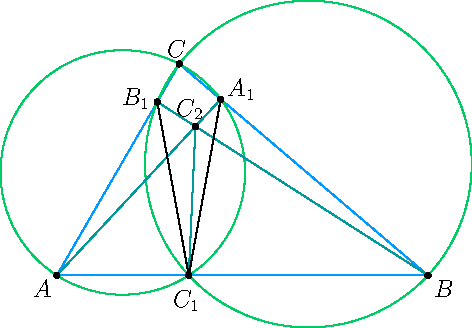
\includegraphics{sharygin-figure.pdf}
  \end{center}

  By power of a point, we observe that $BA_1 = \frac{uc^2}{a}$.
  Therefore, we obtain that
  \[ A_1 = \left( 0:a-\frac{uc^2}{a}: \frac{uc^2}{a} \right)
    = \left( 0:a^{2}-uc^2 : uc^2 \right). \]
  Similarly, $B_1 = \left( b^2-vc^2 : 0 : vc^2 \right)$.
  Therefore,
  \[ C_2 = \left( u(b^2-vc^2) : v(a^2-uc^2) : uvc^2 \right). \]
  Now we show that $C_1$, $C_2$, and $K$ are collinear.
  Expand
  \begin{align*}
  \left\lvert
  \begin{array}{ccc}
    u (b^2-vc^2) & v (a^2-uc^2) & uv c^2 \\
    u & v & 0 \\
    a^2-b^2+c^2 & b^2-a^2+c^2 & -c^2 \\
  \end{array}
  \right\rvert
  &= uvc^2 \left\lvert
  \begin{array}{ccc}
    b^2-vc^2 & a^2-uc^2 & uv \\
    1 & 1 & 0 \\
    \frac{a^2-b^2+c^2}{u} & \frac{b^2-a^2+c^2}{v} & -1 \\
  \end{array}
  \right\rvert \\
  &= uvc^2 \Big[ (a^2-uc^2)-(b^2-vc^2) \\
    &\qquad+ u(b^2-a^2+c^2) - v(a^2-b^2+c^2) \Big] \\
    &= uvc^2 (b^2-a^2)(u+v-1) = 0.
  \end{align*}
\item[p.\  269] in Solution 7.47, delete ``Let $\omega_i$ be the circle with center $O_i$ and radius $r_i$''.
\item[p.\  270] in Solution 7.49, second display, delete ``$\det$''.
\item[p.\  270] in solution 7.52, $T$ should be $au\inv+bv\inv+cw\inv$.
\item[p.\  271] in solution 7.52, the line $PC^2 = \dots$ is missing a plus sign after $-a^2(vw)\inv$.
\item[p.\  271] in solution 7.52, second-to-last display,
  the expressions actually equal $-\gamma$, not $\gamma$.
\item[p.\ 273] Solution 8.31, change ``an reflection'' to ``a reflection''.
\item[pp.\ 273--274] Solution 8.31, swap $A$ and $C$ everywhere, including the figure.
  In addition, $\Psi$ should swap $A$ and $B$ (not fix them).
\item[p.\  274] in Solution 8.31, change ``isogonal with respect to $\angle{BAC}$''
  to ``isogonal with respect to $\triangle{BAC}$''.
\item[p.\  274] Solution 8.36, change ``nine-point circle''
  to ``the nine-point circle'' in third sentence.
\item[p.\  274] \crucial{Solution 8.37 is wrong,
  it assumes $AB$ passes through the center of $\omega_2$.}
\item[p.\  276] in Solution 9.46, the concurrence of lines $IP$ and $EF$
  with the two tangents t the incircle needs justification as well
  (in order to apply Lemma 9.40). It follows from $DEFX$ being harmonic,
  where $X$ is the second intersection of line $AD$ with the incircle.
\item[p.\  276] in Solution 9.47, change $(A,X;B,C)$ to $(A,X;C,B)$.
\item[p.\  277] in Solution 9.50, change $\ol{CG} \cap \ol{BE}$ to $\ol{CG'} \cap \ol{BE}$.
\item[p.\  281] in Solution 10.26, the last line, change $\dang HMN$ to $\dang HNM$.
\item[p.\  282] in Solution 10.29, change $(P,E;X,Y)$ to $(F,E;X,Y)$ in last paragraph.
\item[p.\  282] in Solution 10.30, change ``This solves ... $\dang A_2C_2B_2$'' to
  ``This solves the problem, because the analogous calculation gives $\dang BC_3A_3 = \dang B_2AC$,
  which implies $\dang A_3C_3B_3 = \dang A_3C_3A + \dang AC_3B_3 = \dang A_3C_3B + \dang AC_3B_3
  = \dang CAB_2 + \dang A_2BC = \dang CC_2B_2 + \dang A_2C_2C = \dang A_2C_2B_2$.
  Similarly, we have $\dang B_3A_3C_3 = \dang B_2A_2C_2$ and $\dang C_3B_3A_3 = \dang C_2B_2A_3$.
  Hence $A_3C_3B_3 \sim A_2C_2B_2$ and we are done''.
\item[p.\  286] in Solution 11.6, change ``power'' to ``radius''.
\item[p.\  288] in Solution 11.9, final sentence of second paragraph,
  the tangency is to $(DCM)$, and not $(BCM)$.
\item[p.\  288] in Solution 11.9, last display, change $\frac{KL}{PL}$ to $\frac{PL}{KL}$.
\item[p.\  289] in Solution 11.11, change ``the angle bisector'' to ``an angle bisector''
  and ``the line through $O$ perpendicular to $BC$'' to ``the perpendicular bisector of $BC$''.
\item[p.\  293] in Solution 11.15, change ``the $OPH'$'' to ``$\triangle{OPH'}$''.
\item[p.\  294] delete the dotted circle in solution 11.16, it shouldn't be there.
\item[p.\  295] in Solution 11.17, delete ``(where $A_0$ is the tangency point of the incircle on $BC$)''.
\item[p.\  296] first line, I meant to write $\triangle{AQL}$ and not $(ABL)$
  although these are the same conclusion.
\item[p.\  296] in Solution 11.18, very very end, change $2t$ to $(b^2+c^2)t$.
\item[p.\  297] in Solution 11.18, the first display should read
  $-a^2v + b^2w + c^2v = (b^2+c^2)t + (abc)^2 - (ab)^2S_B - a^2t = S_A ((ab)^2 + 2t)$.
  The next display should be
  $X' = \left( a^2vw : S_A(c^2S_C+t)((ab)^2+2t) : S_A(b^2S_B+t)((ac)^2+2t) \right)$.
  Similarly for $Y'$ and $Z'$.
\item[p.\  297] in Solution 11.19, start of last paragraph, change $DBC_1$ to $DB_1C_1$.
\item[p.\  298] in Solution 11.20, start of solution, define $P$ as the tangency point of $\ell$.
\item[pp.\  298--299] in Solution 11.20, change $\ell_A$, $\ell_B$, $\ell_C$
  to $\ell_a$, $\ell_b$, $\ell_c$, respectively.
\item[p.\  300] in Solution 11.21, the definition of points $T$ and $H'$ are missing.
  Point $T$ is the contact point of the $A$-mixtilinear incircle.
  Point $H'$ is the reflection of $H$ across $M^\ast$.
  Change $I^\ast L^\ast A^\ast$ to $IL^\ast A^\ast$.
\item[p.\  303] in the description of CGMO, ``Girls'' should be ``Girls'\,''.
\item[p.\  303] in the description of IMO, change ``problem'' to ``problems''.
\item[p.\  303] in the description of ELMO, change ``Exceeding'' to ``Exceedingly''.
\item[p.\  305] the link to reference [3] is broken. Fortunately, it's on this website!
  The publication date should be amended to 2012 though.
\item[p.\  305] the link to reference [7] is broken. \url{http://e.math.hr/afine/planegeo.pdf}
  or \url{https://archive.org/details/planegeo} has the file.
\item[p.\  305] reference [10], change ``Geogebral'' to ``Geogebra''.
\end{description}

\end{document}
% vim: nofoldenable textwidth=100
